\clearpage
\section{Getting started}

In this section, we will explain step by step how to get the RAMSES
package and install it, then how to perform a simple test to check the
installation.

\subsection{Obtaining the package}

The package can be downloaded from the Bitbucket repository
\url{https://bitbucket.org/rteyssie/ramses} using the command
\begin{Prompt}
git clone https://bitbucket.org/rteyssie/ramses
\end{Prompt}
You will get a clone of the git repository, with a directory named \dir{trunk/ramses/}.
In this directory, you will find the following directory list:

\begin{Prompt}
README    aton/     doc/      mhd/      pario/    pm/       rt/
amr/      bin/      hydro/    namelist/ patch/    poisson/  utils/
\end{Prompt}

Each directory contains a set of files with a given common purpose. For
example, \dir{amr/} contains all F90 routines dealing with the AMR grid
management and MPI communications, while \dir{hydro/} obviously contains
all F90 routines dealing with hydrodynamics. The first directory you are
interested in is the \dir{bin/} directory, in which the code will be
compiled.

\subsection{Compiling the code}

In this \dir{bin/} directory, you will find a Makefile. The first thing
to do is to edit the Makefile and modify the two variables \cflag{F90}
and \cflag{FFLAGS}. Several examples corresponding to different Fortran
compilers are given. The default values are:

\begin{Prompt}
F90 = gfortran
FFLAGS = -x f95-cpp-input $(DEFINES) -DWITHOUTMPI
\end{Prompt}

The first variable is obviously the command used to invoke the Fortran
compiler. In this case, this is the GNU Fortran compiler. The second
variable contains Fortran flags and preprocessor directives. The last
directive, \cmd{-D}\cflag{WITHOUTMPI}, when used, switches off all MPI
routines. On the other hand, if you don't use this directive, the code
must be linked to the MPI library. We will discuss this point later.
Theses directives are called \emph{Compilation Time Parameters}.  They
should be defined within the Makefile. Default values are:

\begin{Prompt}
NDIM=1
SOLVER=hydro
\end{Prompt}

The first variable, \cflag{NDIM}, sets the dimensionality of the
problem. The default value is for 1D, plan-parallel flows. Allowed
values are 1, 2 and 3. The second directive defines the solver, which in
the current release of RAMSES can be \solver{hydro} or \solver{mhd}.
Other solvers are currently under development, such as a relativistic
solver \solver{rhd}, or a multifluid solver 
\solver{multimat} and so on.

There are 3 other preprocessor directives that can be use in RAMSES:
\cmd{-D\cflag{NVAR}=\cflag{NDIM}+2}, useful to set more variables in the
hydro solver, \cmd{-D\cflag{NPRE}=8}, to set the number of bytes used
for real numbers. \cmd{\cflag{NPRE}=8} corresponds to double precision
arithmetic and \cmd{NPRE=4} to single precision. This option is useful
to save memory during memory intensive runs. Finally, you can use
\cmd{-D\cflag{NVECTOR}=64} to set the size of the vector sweeps for
computationally intensive operations.

To compile RAMSES, execute:

\begin{Prompt}
\$ make
\end{Prompt}

If everything goes well, all source files will be compiled and linked
into an executable called \cmd{ramses1d}.

\subsection{Executing the test case}

To test the compilation, you need to execute a simple test case. Go up
one level and type the following command:

\begin{Prompt}
\$ bin/ramses1d namelist/{\nmlfilename}
\end{Prompt}

The first part of the command is the executable, and the second part, the only
command line argument, is an input file containing all \emph{Run Time
Parameters}. Several examples of such parameter files are given in the
\dir{namelist/} directory. The run we have just performed, \cmd{\nmlfilename},
is the Sod's test, a simple shock tube simulation in 1D. For comparison, we now
show the last {\lastlinescount} lines of standard output:

% TODO : check machine prec here
% NPREC=8
\logfile[\lastlinesln]{autolog/lastlines.log}

To save the standard output in a file, the user is encouraged to
redirect the standard output in a \emph{Log File}, in which all
control variables are outputted and stored, as well as simulation data
for 1D cases only

% TODO: give a reference log in distribution? (make test)
\begin{Prompt}
\$ bin/ramses1d namelist/{\nmlfilename} > {\logfilename}
\end{Prompt}
%
To monitor the progress of longer runs, you can also redirect standard output
to both a log file and the terminal at the same time with:
%
\begin{Prompt}
\$ bin/ramses1d namelist/{\nmlfilename} | tee {\logfilename}
\end{Prompt}

\clearpage % long log file follows !
\subsection{Reading the Log File}
We will now briefly describe the structure and the nature of the
information available in the Log Files. We will use as example the file
\cmd{\logfilename}, which should contain, starting from the top

\logfile{autolog/logstart.log}
%
\hskip 2cm \vdots
%
\logfile[\finestepln]{autolog/finestep.log}

After the code banner and copyrights, the first line indicates that you are
currently using 1 processor and 1 space dimension for this run. The code then
reports that it is building the initial AMR grid. The next lines give the
current mesh structure.

The first level of refinement in RAMSES covers the whole computational domain
with 2, 4 or 8 cells in 1, 2 or 3 space dimensions. The grid is then further
refined up to \nmlentry{levelmin}, which is this case is defined in the
parameter file to be \cmd{levelmin={\nmllevelmin}}.  The grid is then further
refined up to \nmlentry{levelmax}, which is in this case
\cmd{levelmax={\nmllevelmax}}. Each line in the Log File indicates the number
of octs (or grids) at each level of refinement. The maximum number of grids in
each level $l$ is equal to $2^{l-1}$ in 1D, to $4^{l-1}$ in 2D and to $8^{l-1}$
in 3D. The numbers inside parentheses give the minimum, maximum and average
number of grids per processor. This is obviously only relevant to parallel
runs.

The code then indicates the time integration starts. After outputting
the initial conditions to screen, the first \emph{Control Line} appears,
starting with the words \cmd{Fine step=}. The Control Line gives
information on each \emph{Fine Step}, its current number, its current
time coordinate, its current time step. Variable \logentry{a} is for
cosmology runs only and gives the current expansion factor. The last
variable is the percentage of allocated memory currently used by RAMSES
to store each flow variable on the AMR grid and to store each
collision-less particle, if any.

In RAMSES, adaptive time stepping is implemented, which results in defining
\emph{Coarse Steps} and \emph{Fine Steps}. Coarse Steps correspond to the
coarse grid, which is defined by variable \cmd{levelmin}. Fine Steps correspond
to finer levels, for which the time step has been recursively subdivided by a
factor of 2. Fine levels are ``sub-cycled'' twice as more as their parent
coarse level. This explains why, at the end of the Log File, only
{\coarsestepcount} Coarse Steps are reported ({\coarsestepfirst} through
{\coarsesteplast}), for {\finestepcount} Fine Steps (numbered {\finestepfirst}
to {\finesteplast}).

When a Coarse Step is reached, the code writes in the Log File the
current mesh structure. A new Control Line then appears, starting with
the words \cmd{Main step=}. This Control Line gives information on each
Coarse Step, namely its current number, the current error in mass
conservation within the computational box \logentry{mcons}, the current
error in total energy conservation \logentry{econs}, the gravitational
potential energy and the fluid total energy (kinetic plus thermal).

This constitutes the basic information contained in the Log File. In 1D
simulations, output data are also written to standard output, and thus to the
Log File. For 2D and 3D, output data are stored into unformatted Fortran binary
files.  1D data are shown using 5 columns (level of refinement, position of the
cell, density, velocity and pressure) as in the following Sod's test example:

\logfile[\lastoutputln]{autolog/lastoutput.log}

You can cut and paste the {\lastoutputncells} lines into another file and use
your favorite data viewer like \cmd{xmgrace} or \cmd{gnuplot} to visualize the
results.  These should be compared to the plots shown on Figure
\ref{fig:sod1d}. If you have obtained comparable numerical values and levels of
refinements, your installation is likely to be valid. You are encouraged to
edit the parameter file \cmd{\logfilename} and play around with other parameter
values, in order to test the code performances. You can also use other
Parameter Files in the \dir{namelist/} directory.

\begin{figure}
   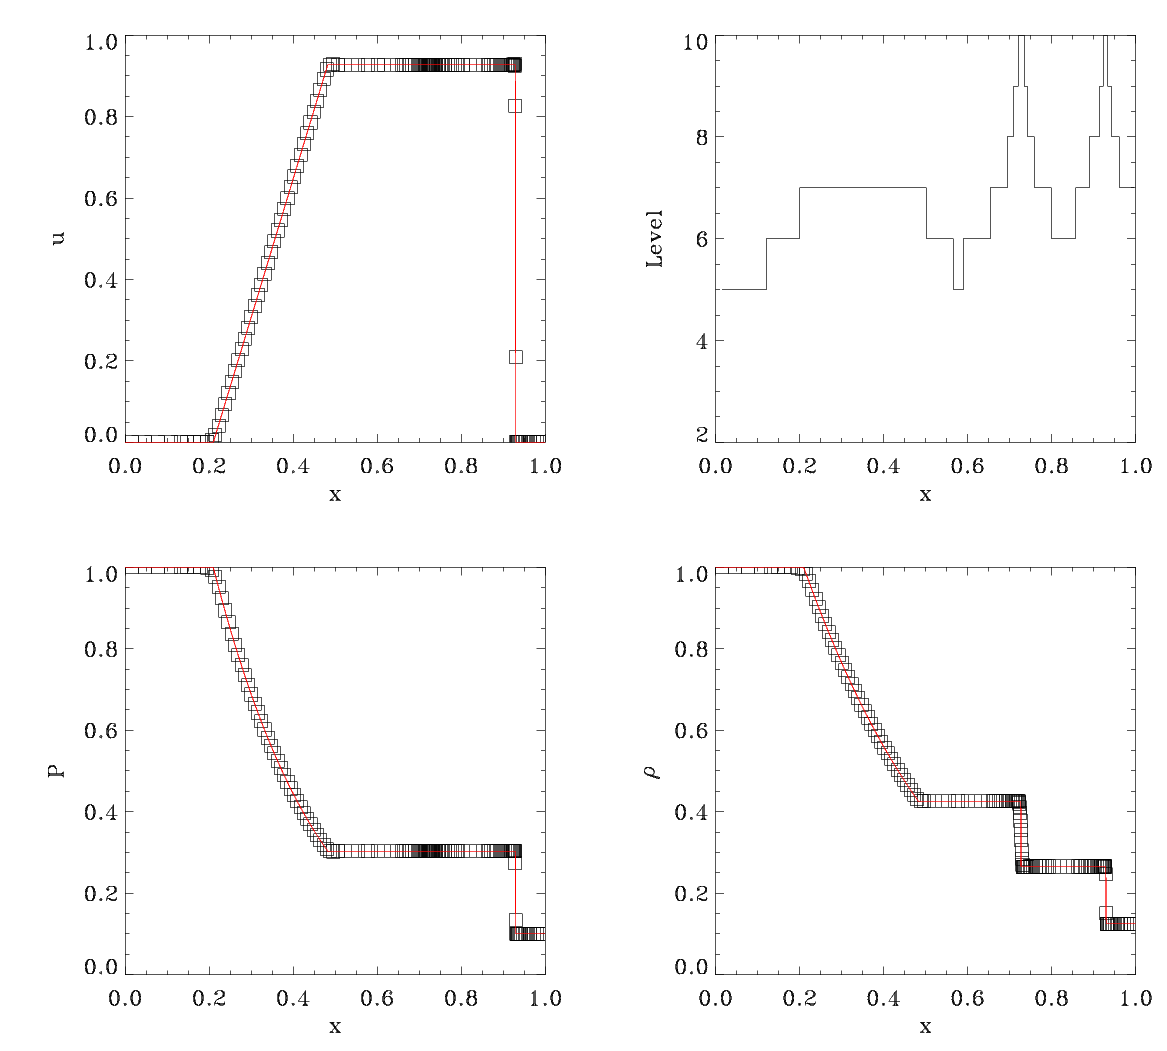
\includegraphics[width=\textwidth]{img/sod.png}
   \caption{Numerical results obtained with RAMSES for the Sod shock
tube test (symbols) compared to the analytical solution (red line).}
   \label{fig:sod1d}
\end{figure}


\begin{warning}
   Do not forget to recompile entirely the code (\cmd{make clean}, then
\cmd{make}) with \cflag{NDIM}\cmd{=2} for 2D cases like \cmd{sedov2d.nml} or
\cmd{NDIM=3} for 3D cases such as \cmd{sedov3d.nml}.
\end{warning}

In the next section, we will describe in more detail the various
Runtime Parameters available within RAMSES.

